\documentclass[12pt]{article}
\usepackage{mathtools}
\usepackage{amsthm}
\usepackage{amsmath}
\usepackage{amssymb}
\usepackage{enumitem}
\usepackage{tikz}
\usepackage{float}
\title{Fourier Polynomials \\ \small from Student Research Projects in Calculus}
\author{Andrew Pringle}
\date{\today}
\newtheorem{conj}{Conjecture}

\begin{document}
\begin{titlepage}
    \centering

    \vspace*{1in}

    {\Huge\bfseries Fourier Polynomials\par}

    \vspace{0.4in}

    {\Large from Student Research Projects in Calculus\par}

    \vspace{1.5in}

    {\LARGE Andrew Pringle\par}

    \vspace{0.5in}

    {\Large \today\par}

    \vspace*{\fill}

\end{titlepage}
This problem was found in the book \textit{Student Research Projects in Calculus} written by Marcus Cohen, Edward D. Guaghan, Arthur Knowbel, Douglas S. Kurtz, and David Penegelley. The problem is named 'Fourier Polynomials'. Below is my proof for the problems presented.

\vspace{.1in}

Let $f$ be a continuous function on the interval $[-\pi,\pi]$. We define the Fourier coefficients of $f$ by the formulae:


\[a_n = \frac{1}{\pi}\int_{-\pi}^{\pi} f(x)\cos(nx) \;\mathrm{d}x\] 
and 
\[ \; b_n = \frac{1}{\pi}\int_{-\pi}^{\pi} f(x)\sin(nx)\; \mathrm{d}x\]

for $n = 0, 1, 2 \dots$ ($n \in \mathbb{N}_0$).

\vspace{.1in}

We also define Fourier polynomials of $f$ to be:

\[P_N(x) = \frac{a_0}{2} + \sum_{n=1}^{N}\left(a_n\cos(nx) + b_n\sin(nx)\right)\]

\vspace{.1in}

Now we begin the problems deemed as 'an introduction to some of Fourier's work'.

\vspace{.1in}

\begin{enumerate}[label=(\alph*)]
    \item Let $f(x) = x$. Find all of the Fourier coefficients of $f$. What are the first five Fourier polynomials $P_N$ associated to $f$? Plot the function f and these five polynomials.
\begin{proof}
    First we let $a = 0$. This will give us:
    \[\frac{1}{\pi}\int_{-\pi}^{\pi}x\; \mathrm{d}x\]
    which will evaluate to $0$ using basic integration. 
    
    \vspace{.1in}
    
    If we let $g(x) =x\cos(nx)$, we can show that $g(x)$ is odd by plugging in $-x$ for $x$:
    \begin{align}
    g(-x) = & (-x)\cos(-nx)
    \\= & -x\cos(nx)
    \\= &-g(x)
    \end{align}

    By proving that $g(x)$ is an odd function, we can conclude that any integral of reflective bounds (in this case, $[-\pi,\pi]$) will be evaluated to $0$.

    \vspace{.1in}

    $\therefore$ \; \; $f(x) = x \implies a_n = 0\ \forall n$

    \vspace{.1in}

    This will simplify our Fourier polynomial definition to:
    \[P_N(x) = \sum_{n=1}^{N}{b_n\sin(nx)}\]

    \vspace{.1in}

    When evaluating $b_1$ - $b_6$ using integration by parts, we are given:

    \[
    \begin{array}{lll}
      b_1 = 2 & b_2 = -1 & b_3 = \dfrac{2}{3} \\
      b_4 = -\dfrac{1}{2} & b_5 = \dfrac{2}{5} & b_6 = -\dfrac{1}{3}
    \end{array}
    \]

    We can notice two patterns for the terms of $2n$ and $2n+1$ as follows:

    \vspace{.1in}

    \[b_{2n+1} = \dfrac{2}{2n+1}\: \:\: \:b_{2n} = -\dfrac{1}{n}\]

    \vspace{.1in}
    
    However, we can find a more concise pattern for both even and odd cases to simplify the formula. Multiplying the numerators and denominators gives

    \vspace{.1in}

    \[
    b_n
    =
    \frac{-2\pi(-1)^n}{\pi n}
    \]

    \vspace{.1in}
    
    Since $\pi$ appears in both the numerator and denominator,
    we can simplify:

    \vspace{.1in}
    
    \[
    b_n
    =
    \frac{-2(-1)^n}{n}
    \]

    \vspace{.1in}
    
    Notice that multiplying $(-1)^n$ by $-1$ increases the exponent
    by one:

    \vspace{.1in}
    
    \[
    -(-1)^n = (-1)^{n+1}
    \]

    \vspace{.1in}
    
    Therefore,

    \vspace{.1in}
    
    \[
    b_n
    =
    \frac{2(-1)^{n+1}}{n}
    \]
    
    \vspace{.1in}
    
    Thus, the Fourier coefficients for $f(x)=x$ are

    \vspace{.1in}
    
    \[
    a_n = 0
    \]
    
    and
    
    \[
    b_n = \frac{2(-1)^{n+1}}{n}
    \]
    
    for all $n \geq 1$.

    \vspace{.1in}

    Our final part of the question asks for the first five Fourier polynomials of $P_N(x)$ along with their graphs on the interval $[-\pi,\pi]$
    \vspace{.1in}
    \[ 
    \begin{array}{l}
        P_1(x) = 2\sin{x} \\ P_2(x) = 2\sin{x} - \sin{2x} \\
        P_3(x) = 2\sin{x} - \sin{2x} + \dfrac{2}{3}\sin{3x} \\ 
        P_4(x) = 2\sin{x} - \sin{2x} + \dfrac{2}{3}\sin{3x} - \frac{1}{2}\sin{4x} \\
        P_5(x) = 2\sin{x} - \sin{2x} + \dfrac{2}{3}\sin{3x} - \dfrac{1}{2}\sin{4x} + \dfrac{2}{5}\sin5x
    \end{array}
    \]
    \begin{figure}[H]
        \centering
        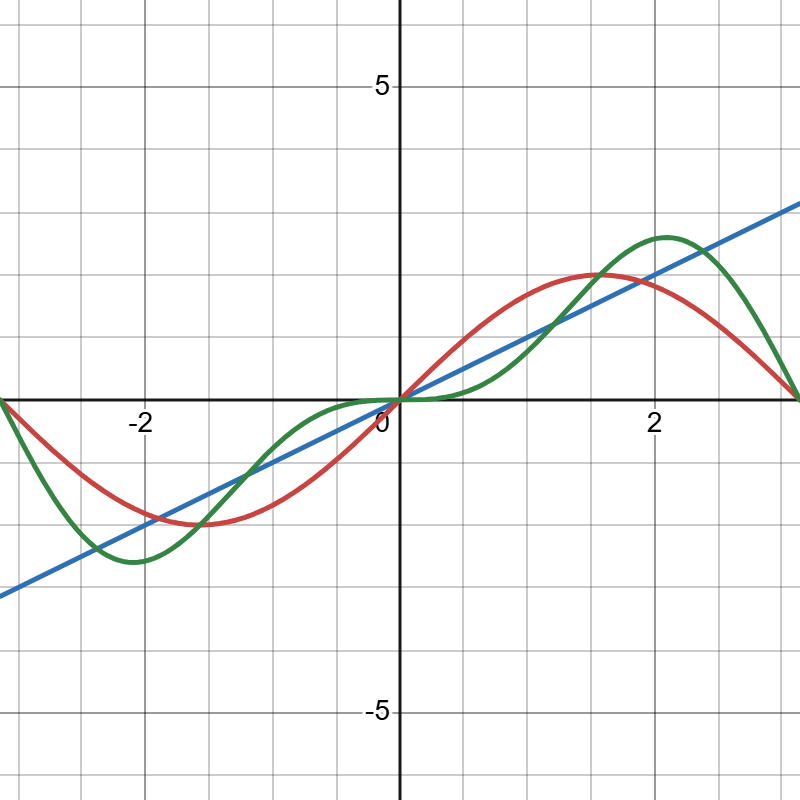
\includegraphics[width=0.25\linewidth]{desmos-graph.png}
        \caption{$x$, $P_1(x)$, $P_2(x)$}
        \label{fig:$x$, $P_1(x)$, $P_2(x)$}
    \end{figure}
    \begin{figure}[H]
        \centering
        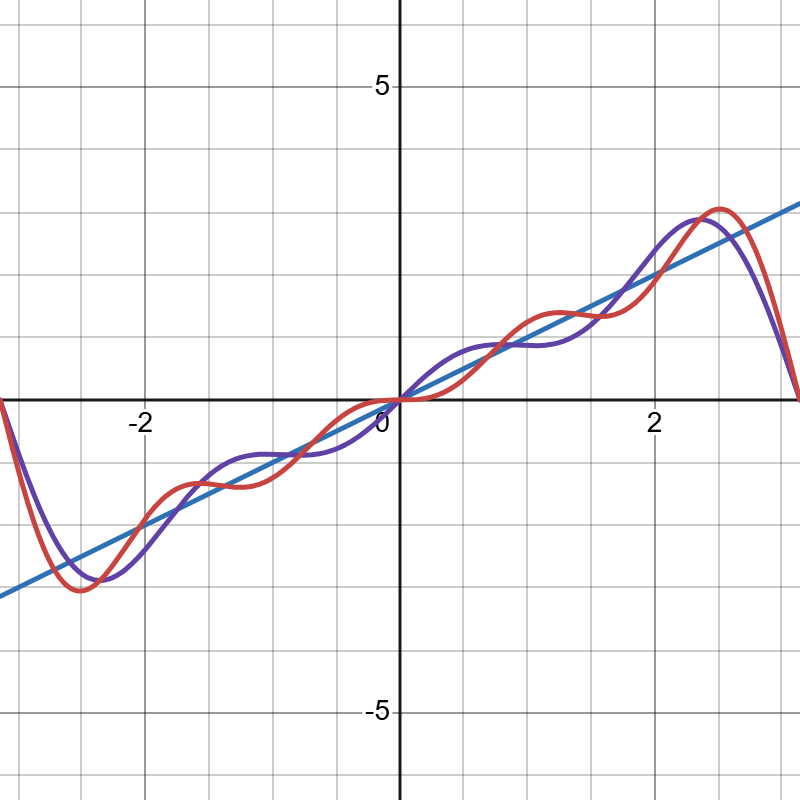
\includegraphics[width=0.25\linewidth]{desmos-graph (1).png}
        \caption{$x$, $P_3(x)$, $P_4(x)$}
        \label{fig:placeholder}
    \end{figure}
    \begin{figure}[H]
        \centering
        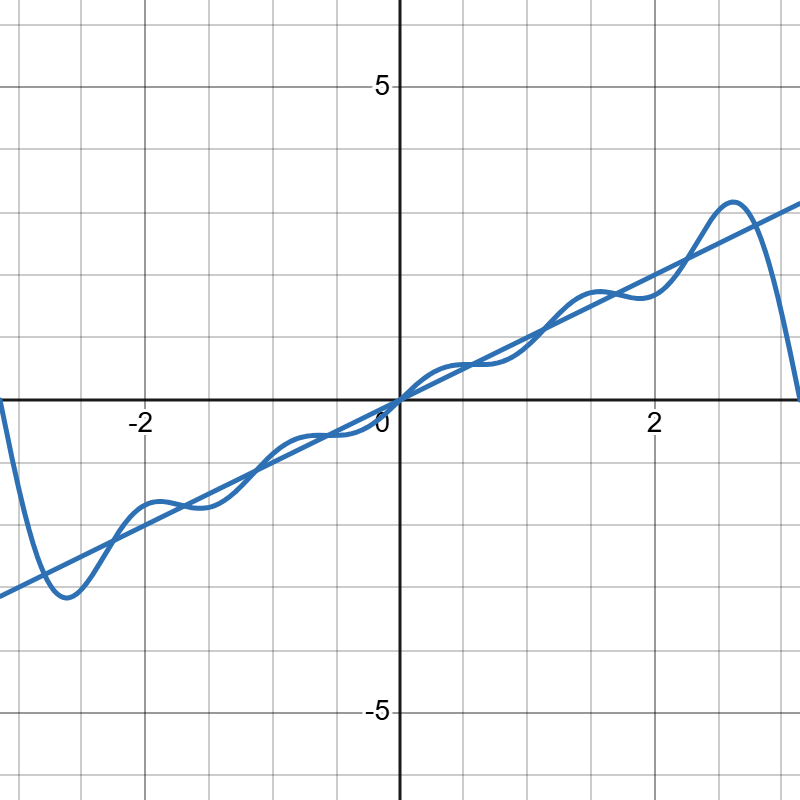
\includegraphics[width=0.25\linewidth]{desmos-graph (2).png}
        \caption{$x$, $P_5(x)$}
        \label{fig:placeholder}
    \end{figure}

    We can see from our graphs that there is an obvious trend of accuracy in approximations.
\end{proof}
\item Let f be an odd function, continuous on the interval $[-c,c]$. Prove that
\[\int_{-c}^{c}f(x)\; \mathrm{d}x = 0\]

\begin{proof}
    \[
        I = \int_{-c}^{c} f(x)\; \mathrm{d}x         = \int_{0}^{c} f(x)\; \mathrm{d}x + \int_{-c}^{0} f(x)\; \mathrm{d}x
    \]
    
    Let
    \[I_2 = \int_{-c}^{0} f(x)\; \mathrm{d}x\]
    Using a u-substitution, we can let $u = -x$, so $du = -dx$. This gives us:
    \[I_2 = \int_{c}^{0}f(-u)\; (-\mathrm{d}u)\]
    
    Since $f(x)$ is an odd function, we know that $f(-x) = -f(x)$. With this information, we can simplify our integral.
    \[\int_{c}^{0}f(u)\; \mathrm{d}u = -\int_{0}^{c}f(u)\; \mathrm{d}u\]

    $u$ is what is called a 'dummy variable', so with a re-substitution of our original $x$ and plugging $I_2$ back into the original integral, we get:
    \[I = \int_{0}^{c}f(x)\; \mathrm{d}x + \left(-\int_{0}^{c}f(x)\; \mathrm{d}x\right)\]
    \[= 0\]
    
    \vspace{.1in}
    \[\therefore \int_{-c}^{c}f(x)\; \mathrm{d}x = 0\]
\end{proof}
\item In part (a), something special happened because the function, $f(x) = x$, is an odd function on $[-\pi,\pi]$. What pattern did you notice? Next, let $f$ be any odd function on $[-\pi,\pi]$. Make a conjecture about the Fourier coefficients of $f$. Prove your conjecture.

\begin{conj}
    For any odd function $f(x)$, the $a_n$ Fourier coefficients will be $0$.
\end{conj}
\vspace{.1in}
\begin{proof}
We compute
\[
a_n = \frac{1}{\pi}\int_{-\pi}^{\pi} f(x)\cos(nx)\,dx
\]
where $f(x)$ is odd and $\cos(nx)$ is even.

\vspace{.1in}

Let
\[
g(x)=f(x)\cos(nx)
\]

Then
\[
g(-x)=f(-x)\cos(-nx)
\]

Since $f(x)$ is odd and $\cos(nx)$ is even,
\[
f(-x)=-f(x), \quad \cos(-nx)=\cos(nx)
\]

Thus
\[
g(-x)=-f(x)\cos(nx)=-g(x)
\]

So $g(x)$ is an odd function.

\vspace{.1in}

Therefore,
\[
\int_{-\pi}^{\pi} g(x)\,dx = 0
\quad \Rightarrow \quad
a_n = 0
\] 
$ \forall n \geq 1$.


\vspace{.1in}

Hence, all cosine coefficients vanish for any odd function.
\end{proof}


\item Another special collection of functions on an interval $[-c,c]$ is the even functions. After thinking about what happens for the odd functions, make a conjecture about the Fourier coefficients of an even function. Let $f(x) = x^2$; check your conjecture using this even function. Explain why your conjecture is true for any function.

\vspace{.1in}
For this part, we will combine a similar approach to what we have done in both parts (a) and (c).
\begin{conj}
    For any even function $f(x)$, the $b_n$ Fourier coefficients will be $0$ and $a_n$ coefficients will $\neq 0$.
\end{conj}

\begin{proof}
    Recall that 
    \[P_N(x) = \dfrac{a_0}{2} + \sum_{n=1}^{N}a_n\cos({nx}) + b_n\sin({nx})\]

    We will first  evaluating $a_n$ coefficients of $a_0$ through $a_5$.

    \[
    \begin{array}{lll}
      a_0 = \dfrac{2\pi^2}{3} & a_1 = -4 & a_2 = 1 \\
      a_3 = -\dfrac{4}{9} & a_4 = \dfrac{1}{4} & a_5 = -\dfrac{4}{25}
    \end{array}
    \]

    Notice that the term $(-1)^n$ alternates signs depending on whether
    $n$ is even or odd:
    
    \[(-1)^n =
    \begin{cases}
    1 & \text{if $n$ is even} \\
    -1 & \text{if $n$ is odd}
    \end{cases}
    \]
    
    \vspace{.1in}
    
    Now consider the formula
    
    \[a_n = \frac{4(-1)^n}{n^2}\]
    
    We verify this formula for both even and odd cases.
    
    \vspace{.1in}
    
    If $n$ is even, then $(-1)^n = 1$, so
    
    \[ a_n = \frac{4(1)}{n^2} = \frac{4}{n^2}\]
    
    For example,
    
    \[a_2 = \frac{4}{2^2} = 1\]
    
    and
    
    \[
    a_4
    =
    \frac{4}{4^2}
    =
    \frac14
    \]
    
    which agrees with the even coefficients above.
    
    \vspace{.1in}
    
    If $n$ is odd, then $(-1)^n = -1$, so
    
    \[a_n = \frac{4(-1)}{n^2} = -\frac{4}{n^2}\]
    
    For example,
    
    \[a_1 = -\frac{4}{1^2} = -4\]
    
    and
    
    \[a_3 = -\frac{4}{3^2} = -\frac49\]
    
    which agrees with the odd coefficients above.
    
    \vspace{.1in}
    
    Therefore, both cases may be summarized by the compact formula
    
    \[a_n = \frac{4(-1)^n}{n^2}\]
    
    for all $n \geq 1$.

    \vspace{.1in}

    As we found $a_0$. we can simplify $P_N(x)$
    \[P_N(x) = \dfrac{\pi^2}{3}\ + \sum_{n=1}^{N}a_n\cos({nx}) + b_n\sin({nx})\]

    Since $f(x)$ is even and $\sin(nx)$ is odd, their product
    $f(x)\sin(nx)$ is an odd function. Therefore,
    
    \[b_n = \frac{1}{\pi}\int_{-\pi}^{\pi} f(x)\sin(nx)\,dx = 0.\] 
    
    Using this information, we can make a broader claim to the conjecture we made earlier that any even function will allow $b_n$ to always = 0.

    \vspace{.1in}

    If we let $f(x)$ be any even function, our $b_n$ coefficient is defined as:

    \[\dfrac{1}{\pi}\int_{-\pi}^{\pi}f(x)\sin({nx}) \; \mathrm{d}x\]
    \vspace{.1in}
    Let 
    \begin{align}
        g(x) = & f(x)\sin({nx}) \\
        g(-x) = & f(-x)\sin(-nx)
    \end{align}

    This is almost an exact opposite case of what we saw in part (c), rather $f(x)$ is defined as an even function, and $\sin{x}$ is a known odd function. 

    \begin{align}
        = & -f(x)\sin(nx)
        = - g(x)
    \end{align}

    This proves that $g(x)$ is an odd function. Using what we learned from part (b), we can determine that every $b_n$ coefficient will evaluate to 0 when f(x) is an even function.
    
    
\end{proof}
    
\end{enumerate}

\end{document}
